\documentclass[a4paper,11pt]{article}

\input ../include/preamble.tex

% Finite state machines
\usepackage{tikz}
\usetikzlibrary{arrows, automata, topaths, calc, shapes.geometric}

% SECTIONS
%
% * Introduction
% * AVL trees
% * Single rotate
% * Double rotate
% * All the rotations
% * The implementation
% * Insert
% * Rotation
% * Single rotation
% * Double rotations
% * Benchmarks


\begin{document}

% ================================================== %
% == Title  == %
% ================================================== %

\title{
    \textbf{AVL Trees}\\
    \large{Programming II - Elixir Version}
}
\author{Johan Montelius}
\date{Spring Term 2018}
\maketitle
\defaultpagestyle


% ================================================== %
% == Introduction  == %
% ================================================== %

\section*{Introduction}

In this assignment you're going to implement operations on what is
called an AVL tree. An AVL tree is a fairly well balanced sorted
binary tree where the depth of two branches will differ by at most
one. Searching in the tree is straight forward but when we add an
element to the tree we might have to re-arrange the nodes to preserve
the AVL property. The general idea how nodes are rearranged is easy to
explain if you leave out the details; the devil is of course in the
details.


% ================================================== %
% == AVL trees  == %
% ================================================== %

\section{AVL trees}

AVL trees are named after two Russian mathematicians, Georgy
Adelson-Velsky and Evgenii Landis, who first described how we could
rearrange a binary search tree in constant time in each insert
operation to keep it balanced. The idea is of course to keep the
look-up operations to $O(lg(n))$ and avoid the worst case $O(n)$
scenarios that we could have if the tree becomes to imbalanced.

The trick is to keep track of the difference in depth of branches so
each node will be augmented with a flag to signal that the left branch
is deeper ($-1$), the two branches are of equal depth ($0$) or if the
right branch is deeper ($+1$). When we insert a new node in the tree we
could temporarily have a situation where a node is labeled with $-2$ or
$+2$. This would violate the AVL property and is therefore immediately
mitigated by a {\em rotation}. The rotation must of course preserve
the ordering but still remove the violating imbalance. The different
rotation operations are not tricky {\em per se} but there are many
cases to keep track of so it's very easy to do mistakes. 

We will first look at the two basic rotations that we will do and then
dig deeper into the details of how to implement them.


% ================================================== %
% == Single rotate  == %
% ================================================== %

\section{Single rotate}

The single rotate operation is performed when the left-left branch or
right-right branched has increased with one step and causes an
imbalance. The left-left station is shown in
figure~\ref{fig:single}. The depth of the sub-tree A is one greater
than the sub-tree of B and also two greater than the sub-tree of C. In
the rearranged tree, the branches are balanced and the total depth of
the tree is one less than the imbalanced tree.

The left-left single rotation has its mirror in the right-right
single rotation used when the root has a difference of $+2$ and the
right sub-tree a difference of $+1$.

\begin{figure}[h!]

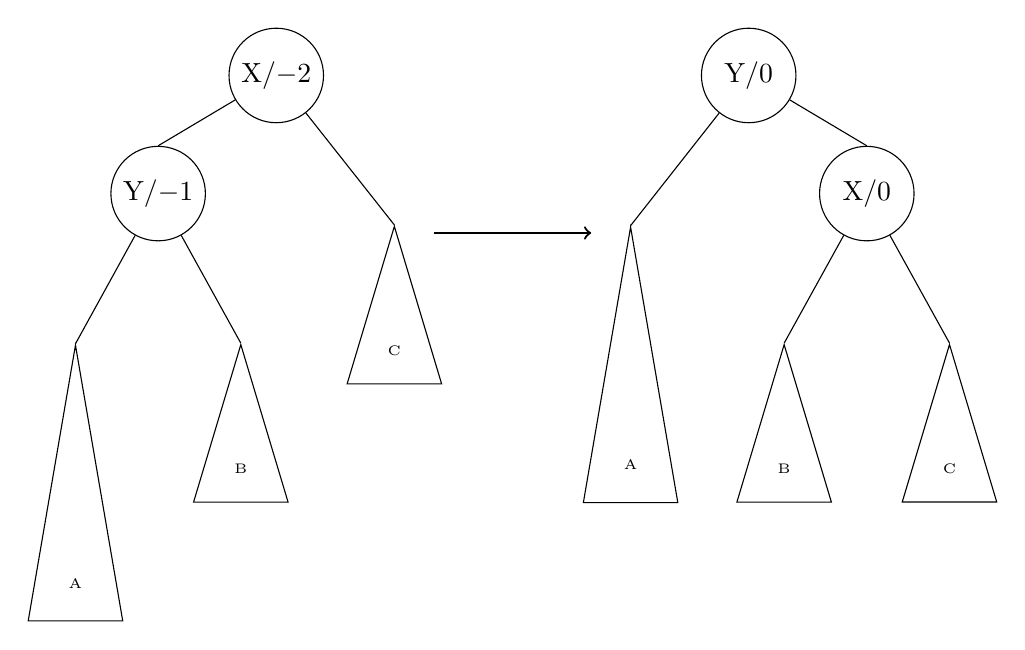
\begin{tikzpicture}[
    inner/.style={circle,draw,minimum width=12mm,inner sep=1pt},
    leaf/.style={isosceles triangle,draw,shape border rotate=90,isosceles triangle stretches=true, minimum height=20mm,minimum width=12mm,inner sep=0,yshift={-20mm},font=\tiny},
    large leaf/.style={leaf,minimum height=35mm,yshift={-14.5mm}},
    level 1/.style={sibling distance=30mm},
    level 2/.style={sibling distance=21mm},
    level 3/.style={sibling distance=14mm}]

    \node[inner] at (2,4)  {X/$-2$}
    [child anchor=north]
    child {node[inner] {Y/$-1$}
        child {node[large leaf] {A}}
        child {node[leaf] {B}}}
    child {node[leaf] {C}};

    \draw[thick, ->] (4,2) -- (6,2);

    \node[inner] at (8,4)  {Y/$0$}
    [child anchor=north]
    child {node[large leaf] {A}}
    child {node[inner] {X/$0$}
        child {node[leaf] {B}}
        child {node[leaf] {C}}};
\end{tikzpicture}

\caption{Single rotation: the left-left branch has grown and caused an imbalance. \label{fig:single}}
\end{figure}


% ================================================== %
% == Double rotate  == %
% ================================================== %

\section{Double rotate}

In the double rotate we have added an element in the left-right branch
(or the right-left branch). There are three different flavors of this
rule depending on what the left-right branch looks like. The first
rule is shown in figure~\ref{figure:double} and shows the situation
where the left-right branch is marked with $-1$. This is the case where
the left-right-left branch (B) has been extended. Note the difference
in depth of the sub-trees, A has to be of the same depth as B and D
and C must be one level shorter.

The second version of this rule covers the situation where the
left-right-left branch is marked with $+1$ i.e. the sub-tree C is deeper
than the sub-tree B. The same transformation is done but the resulting
depth differences are of course different. You're encouraged to write
this rule down since you will use it in the implementation.

\begin{figure}[h!]
    
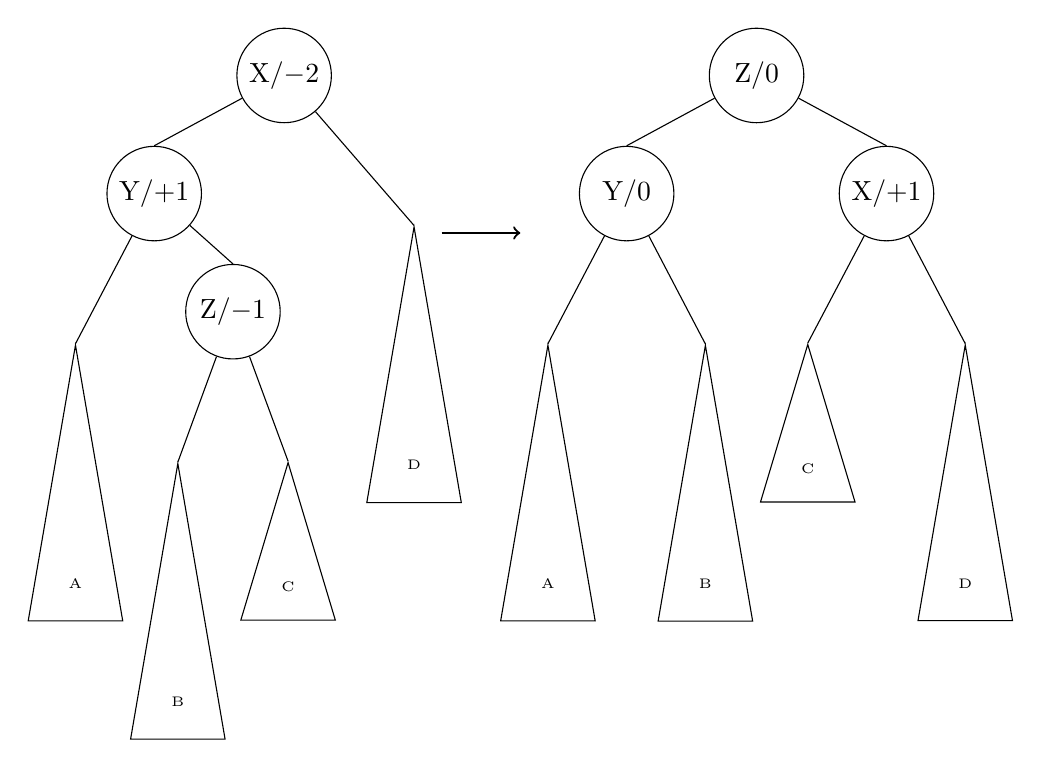
\begin{tikzpicture}[
    inner/.style={circle,draw,minimum width=12mm,inner sep=1pt},
    leaf/.style={isosceles triangle,draw,shape border rotate=90,isosceles triangle stretches=true, minimum height=20mm,minimum width=12mm,inner sep=0,yshift={-20mm},font=\tiny},
    large leaf/.style={leaf,minimum height=35mm,yshift={-14.5mm}},
    level 1/.style={sibling distance=33mm},
    level 2/.style={sibling distance=20mm},
    level 3/.style={sibling distance=14mm}]

    \node[inner] at (2,4)  {X/$-2$}
    [child anchor=north]
    child {node[inner] {Y/$+1$}
        child {node[large leaf] {A}}
        child {node[inner] {Z/$-1$}
        child {node[large leaf] {B}}
        child {node[leaf] {C}}}}
    child {node[large leaf] {D}};

    \draw[thick, ->] (4,2) -- (5,2);

    \node[inner] at (8,4)  {Z/$0$}
    [child anchor=north]
    child { node[inner] {Y/$0$} 
        child {node[large leaf] {A}}
        child {node[large leaf] {B}}}
    child {node[inner] {X/$+1$}
        child {node[leaf] {C}}
        child {node[large leaf] {D}}};
\end{tikzpicture}

\caption{Double rotation: the left-right branch has grown and caused an imbalance. \label{fig:double}}
\end{figure}

The third version of this rule is a special case where the
left-right-left sub-tree is marked with 0. This only happens if node Z
is the element that was added to the tree (a leaf node has two empty
sub-trees and the difference is then 0). If the depth of the sub-trees
of Z is zero then the also the depth of A and D must be zero. If all
sub-trees are of depth zero then of course the nodes of the
transformed tree all have a depth difference of 0.

In the implementation we will have a choice whether we should handle
this special situation when it occurs or just use a general scheme
that works in all cases. We will use the general approach to make the
implementation as easy to follow as possible but one could keep this
in mind if we want to improve the performance of the implementation.


% ================================================== %
% == All the rotations  == %
% ================================================== %

\section{All the rotations}

One thing that is important to note is that the maximum depth of the
tree after the rotation is one less than before the rotation. We will
use this fact in the implementation when we keep track of depth
differences in the recursive operations.

All in all there are eight rotations that we will have to
implement. There are two single rotations, left ad right, and these
are quite straight forward. The three left-right and three right-left
are trickier since we have to get the depth differences right. If you
draw the transformations graphs of these rules you're more likely to
get it right, if you think you can hold these rules in your head, I
can only wish you good luck - you'll need it :-)


% ================================================== %
% == The implementation  == %
% ================================================== %

\section{The implementation}

Ok, let's go how hard can this be. Let's start by defining the
data structure to represent a tree. We're going to use a tuple with: a
key and value, a depth difference and a left and right branch. An
empty tree or empty branch is represented by {\tt nil} and there is
no special representation of leaf nodes.

\begin{itemize}
\item {\tt \{:node, key, value, diff, left, right\}}
\item {\tt nil}
\end{itemize}


% ================================================== %
% == Insert  == %
% ================================================== %

\section{Insert}

We will implement an insertion function that will take an AVL tree, a
key and value and return an AVL tree where the key-value pair has been
added or, if it existed, updated. In the recursive implementation of
the insertion function we will need to keep track of when the depth of
a sub-tree changes and update the depth differences accordingly. We
therefor us an internal function {\tt insrt/3} that returns either
{\tt\{:ok, t\}} if the resulting tree is of equal depth or, {\tt
\{:inc, t\}} if the depth has been increased by one (the depth can only
increase by at most one).

\begin{minted}{elixir}
def insert(tree, key, value) do
    case insrt(tree, key, value) do
    {:inc, q} -> q
    {:ok, q} -> q
    end
end
\end{minted}

The implementation of the {\tt insrt/3} function has two special cases
and six general rules, three for each branch. The two special cases if
of course if the tree is empty or if we find the key in the root of
the tree. Note that we in the first case return a tuple that indicates
that the tree has grown by one level.

\begin{minted}{elixir}
defp insrt(nil, key, value) do
    {:inc, {:node, key, value, 0, nil, nil}} 
end

defp insrt({:node, key, _, f, a, b}, key, value) do
    {:ok, {:node, key, value, f, a, b}}
end
\end{minted}

In the general case we have to go down either the left branch or the
right branch but now we have several alternatives depending on the
depth difference of the root node and weather or not the insertion of
the key-value pair increases the depth of the branch. We will first
look at the simple cases and leave the two problematic cases until the end.

If the tree is balanced and we are going down the left branch either
of two things can happened: the depth of the left branch is incremented
by one or its depth remains the same. If it does increase we must of
course return a structure that indicates that the depth of the
resulting tree has increased. We also provide the correct depth
difference that now is $-1$.

\begin{minted}{elixir}
defp insrt({:node, rk, rv, 0, a, b}, kk, kv) when kk < rk do
    case insrt(a, kk, kv) do
    {:inc, q} ->
        {:inc, {:node, rk, rv, -1, q, b}}
    {:ok, q} ->
        {:ok, {:node, rk, rv, 0, q, b}}
    end
end
\end{minted}

This rule of course has its right counter part; which branch should we
go down, what should we do if the depth of that branch is increased,
what is the resulting depth difference?

The second alternative is if we're going down the left branch but in a
tree that has a deeper right branch. This case is almost the same but
now we will not increase the total depth of the tree even if we
increase the depth of the left branch. This rule also has its
right counterpart and the difference is minute (but oh how important).

\begin{minted}{elixir}
defp insrt({:node, rk, rv, +1, a, b}, kk, kv) when kk < rk do
    case insrt(a, kk, kv) do
    {:inc, q} ->
        {:ok, {:node, rk, rv, 0, q, b}}
    {:ok, q} ->
        {:ok, {:node, rk, rv, +1, q, b}}
    end
end
\end{minted}

The tricky case comes when we're going down the left or right branch
and this is already a branch that is longer than its sibling. In this
case we could end up in a situation were have a depth difference of
2. This is were we rely on our {\em rotator} to fix things for us. 
Note that
the rotation will result in a tree that does not change the maximum
depth of the original tree. After a rotation we can safely return the
result as it is without any warning that the depth has increased.

\begin{minted}{elixir}
defp insrt({:node, rk, rv, -1, a, b}, kk, kv) when kk < rk do
    case insrt(a, kk, kv) do
    {:inc, q} ->
        {:ok, rotate({:node, rk, rv, -2, q, b})}
    {:ok, q} ->
        {:ok, {:node, rk, rv, -1, q, b}}
    end
end
\end{minted}

If you also implement the final right branch version of this last rule
you have completed all the rules needed. We of course have the problem
of describing the rotations but this is more of a pattern matching
exercise if you have drawn all the graphs.


% ================================================== %
% == Rotation  == %
% ================================================== %

\section{Rotation}

Can you provide a better strategy for the philosophers so that they
can eat and dream without ending up in a deadlock? What happens if
you provide a waiter that controls how many philosophers that can eat
at any given time. How would this help the situation? How many
philosophers can try to eat without ending up in a deadlock? How
smart does the waiter need to be?


% ================================================== %
% == Single rotation  == %
% ================================================== %

\section{Single rotation}

Let's start with the simple cases were we can use a simple
rotation. If the root is annotated with $-2$ and the left branch is
annotated with $-1$ we can do a rotation of the left branch. If its the
opposite we do a rotation of the right branch.

\begin{minted}{elixir}
defp rotate({:node, xk, xv, -2, {:node, yk, yv, -1, a, b}, c}) do
    {:node, yk, yv, 0, a, {:node, xk, xv, 0, b, c}}	    
end

defp rotate({:node, xk, xv, +2, a, {:node, yk, yv, +1, b, c}}) do
    {:node, yk, yv, 0, {:node, xk, xv, 0, a, b}, c}
end
\end{minted}

Note how the first rule is a direct mapping if the graph in
figure~\ref{fig:single}. If we know that the drawn rule is correct
there is little room for doing any mistakes i.e. if the logic is right
the coding is trivial.


% ================================================== %
% == Double rotations  == %
% ================================================== %

\section{Double rotations}

The double rotations are of course more complicated but the
complication is more in geting the logic right and not in the
implementations. We can first look at the rule that is described in
figure~\ref{fig:double}. We know what the tree should look like and we
know what the result should be.

\begin{minted}{elixir}
defp rotate({:node, xk, xv, -2, {:node, yk, yv, +1, a, 
{:node, zk, zv, -1, b, c}}, d}) do
    {:node, zk, zv, 0, {:node, yk, yv, 0, a, b}, {:node, xk, xv, +1, c, d}}
end
\end{minted}

The second rule covers the case where the Z node has a right branch
that is deeper than its left branch. If you have drawn the trees the
implementation of the rule should be straight forward.

\begin{minted}{elixir}
defp rotate({:node, xk, xv, -2, {:node, yk, yv, +1, a, 
{:node, zk, zv, +1, b, c}}, d}) do
    {:node, zk, zv, 0, {:node, yk, yv, -1, a, b}, {:node, xk, xv, 0, c, d}}
end
\end{minted}

The last of the left-right rules is the one that handles the special
case where the two branches of the Z node are of equal
length. Remember that this was a very special case and if we can
detect this earlier we might do without this rule all together.

\begin{minted}{elixir}
defp rotate({:node, xk, xv, -2, {:node, yk, yv, +1, a, 
{:node, zk, zv, 0, b, c}}, d}) do
    {:node, zk, zv, 0, {:node, yk, yv, 0, a, b}, {:node, xk, xv, 0, c, d}}
end
\end{minted}

The three left-right rules of course have their right-left counterparts
but these are all left for the reader as an exercise. One advice is to
draw the rules first and only then implement them. It's very easy to
mix up a $-1$ for a $+1$ or swap a left branch for a right branch. If
you draw the rules first it should not be a problem.


% ================================================== %
% == Benchmarks  == %
% ================================================== %

\section{Benchmarks}

The whole idea with AVL trees is that we should gain some performance
so let's do some benchmarks to see if all the trouble was worth the
effort. After all, if the performance gain is not enough it might be
better to have less code to make it easier to verify that we have done
the right thing.

In order to evaluate our implementation we could generate a tree from
a sequence of keys and then see what the tree looks like and compare
it to a tree generated by the regular binary sorted tree
algorithms. What is interesting is if the AVL tree is more balanced
i.e. that the average depth at which we will find our keys is small. A
perfectly balanced tree will have a depth of $lg(n)$ and it's
interesting to see how close to this that the AVL tree is.

Let's create two modules, {\tt Avl} and {\tt Bst}, that implements the
following functions:

\begin{itemize}
\item {\tt tree()} : returns an empty tree.
\item {\tt insert(tree, key, value)} : returns a tree where the key value has been inserted (or updated if key existed).
\item {\tt depth(tree, key)} : returns {\tt \{:ok, depth\}}, with the depth at which the key is found, or {\tt :fail} if the key is not found.
\item {\tt max\_depth(tree)} : returns the maximum depth of the tree. 
\end{itemize}

We will use the {\tt depth/2} function to both gather statistics on the
depth at which keys are found and also measure the time it takes to
find a key. The depth function will of course do exactly the same
steps as a {\tt lookup/2} function would do.

Let's now in a module called {\tt Test} implement some benchmarks that
compares the {\tt Avl} and {\tt Bst} module. The first thing wee need
is a function that generates a sequence of keys in random order. We
will use this sequence to first build a tree and then examine how long
time it takes to access the keys. Define a function {\tt
    sequence(n, m)} that generates a list of $n$ integers from $1$ to $m$
(we're using the Erlang library module {\tt random}).

\begin{minted}{elixir}
defp sequence(0, _), do: []

defp sequence(i, t), do: [:rand.uniform(t) | sequence(i - 1, t)]
\end{minted}

\end{document}
    
